\chapter{与视频无关的干扰:有效的针对孪生视觉跟踪的有针对性的攻击} \label{chap:attack}

\section{摘要}
在前面的章节中,我们展示了通过添加时空信息、语义信息和自适应信息,可以有效提高视频跟踪算法的性能。然而,最近显示,孪生追踪器容易受到对抗性攻击。但是,现有的攻击方法独立地为每个视频制作扰动,这在计算上是不可忽略的。问题是,如果我们在现实世界的在线跟踪阶段无法访问有限的计算资源,该怎么办?

在本文中,我们展示了与视频无关的扰动的存在,这些扰动可以使有针对性的攻击成为可能,例如,强制跟踪器遵循具有指定偏移量的地面真相轨迹,使其具有通用性并且不受网络中的推理影响。具体来说,我们通过向模板图像添加通用的不可感知的扰动并将 \textit{虚假目标}(即小的通用对抗补丁)粘贴到符合预定义轨迹的搜索图像中来攻击跟踪器,以便跟踪器输出 \textit{虚假目标} 的位置和大小,而不是实际目标。我们的方法允许仅通过添加和粘贴操作就可以干扰新颖的视频,而无需支付额外的费用,并且不需要进行梯度优化或网络推理。在多个数据集上的实验结果表明,我们的方法可以以有针对性的攻击方式有效地欺骗孪生跟踪器。我们将使我们的代码公开可用。

\section{简介}

\begin{figure}[t]
\centering
\subfloat{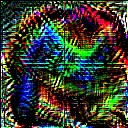
\includegraphics[width=0.3\textwidth]{Img/attack/x.jpg}} \qquad 
\subfloat{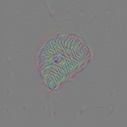
\includegraphics[width=0.3\textwidth]{Img/attack/z.jpg}}
\caption{补丁可视化结果。}
\end{figure}

给定初始视频帧中的任意检测到或注释的关注对象,视觉对象跟踪的目标是识别并定位同一对象在后续帧中的其他实例。在线跟踪阶段中从单个初始样本跟踪视觉对象的这种范式最近被广泛地描述为基于孪生网络的单发问题 \cite{SiamFC,SiamRPN,SiamRPN++,SiamFC++},称为孪生视觉跟踪,并被认为对视觉跟踪非常有效。

\begin{figure}[thbp]
\centering
%\subfigure{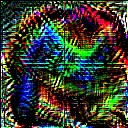
\includegraphics[width=0.2\textwidth]{Img/attack/x.jpg}} \qquad
%\subfigure{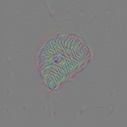
\includegraphics[width=0.2\textwidth]{Img/attack/z.jpg}}
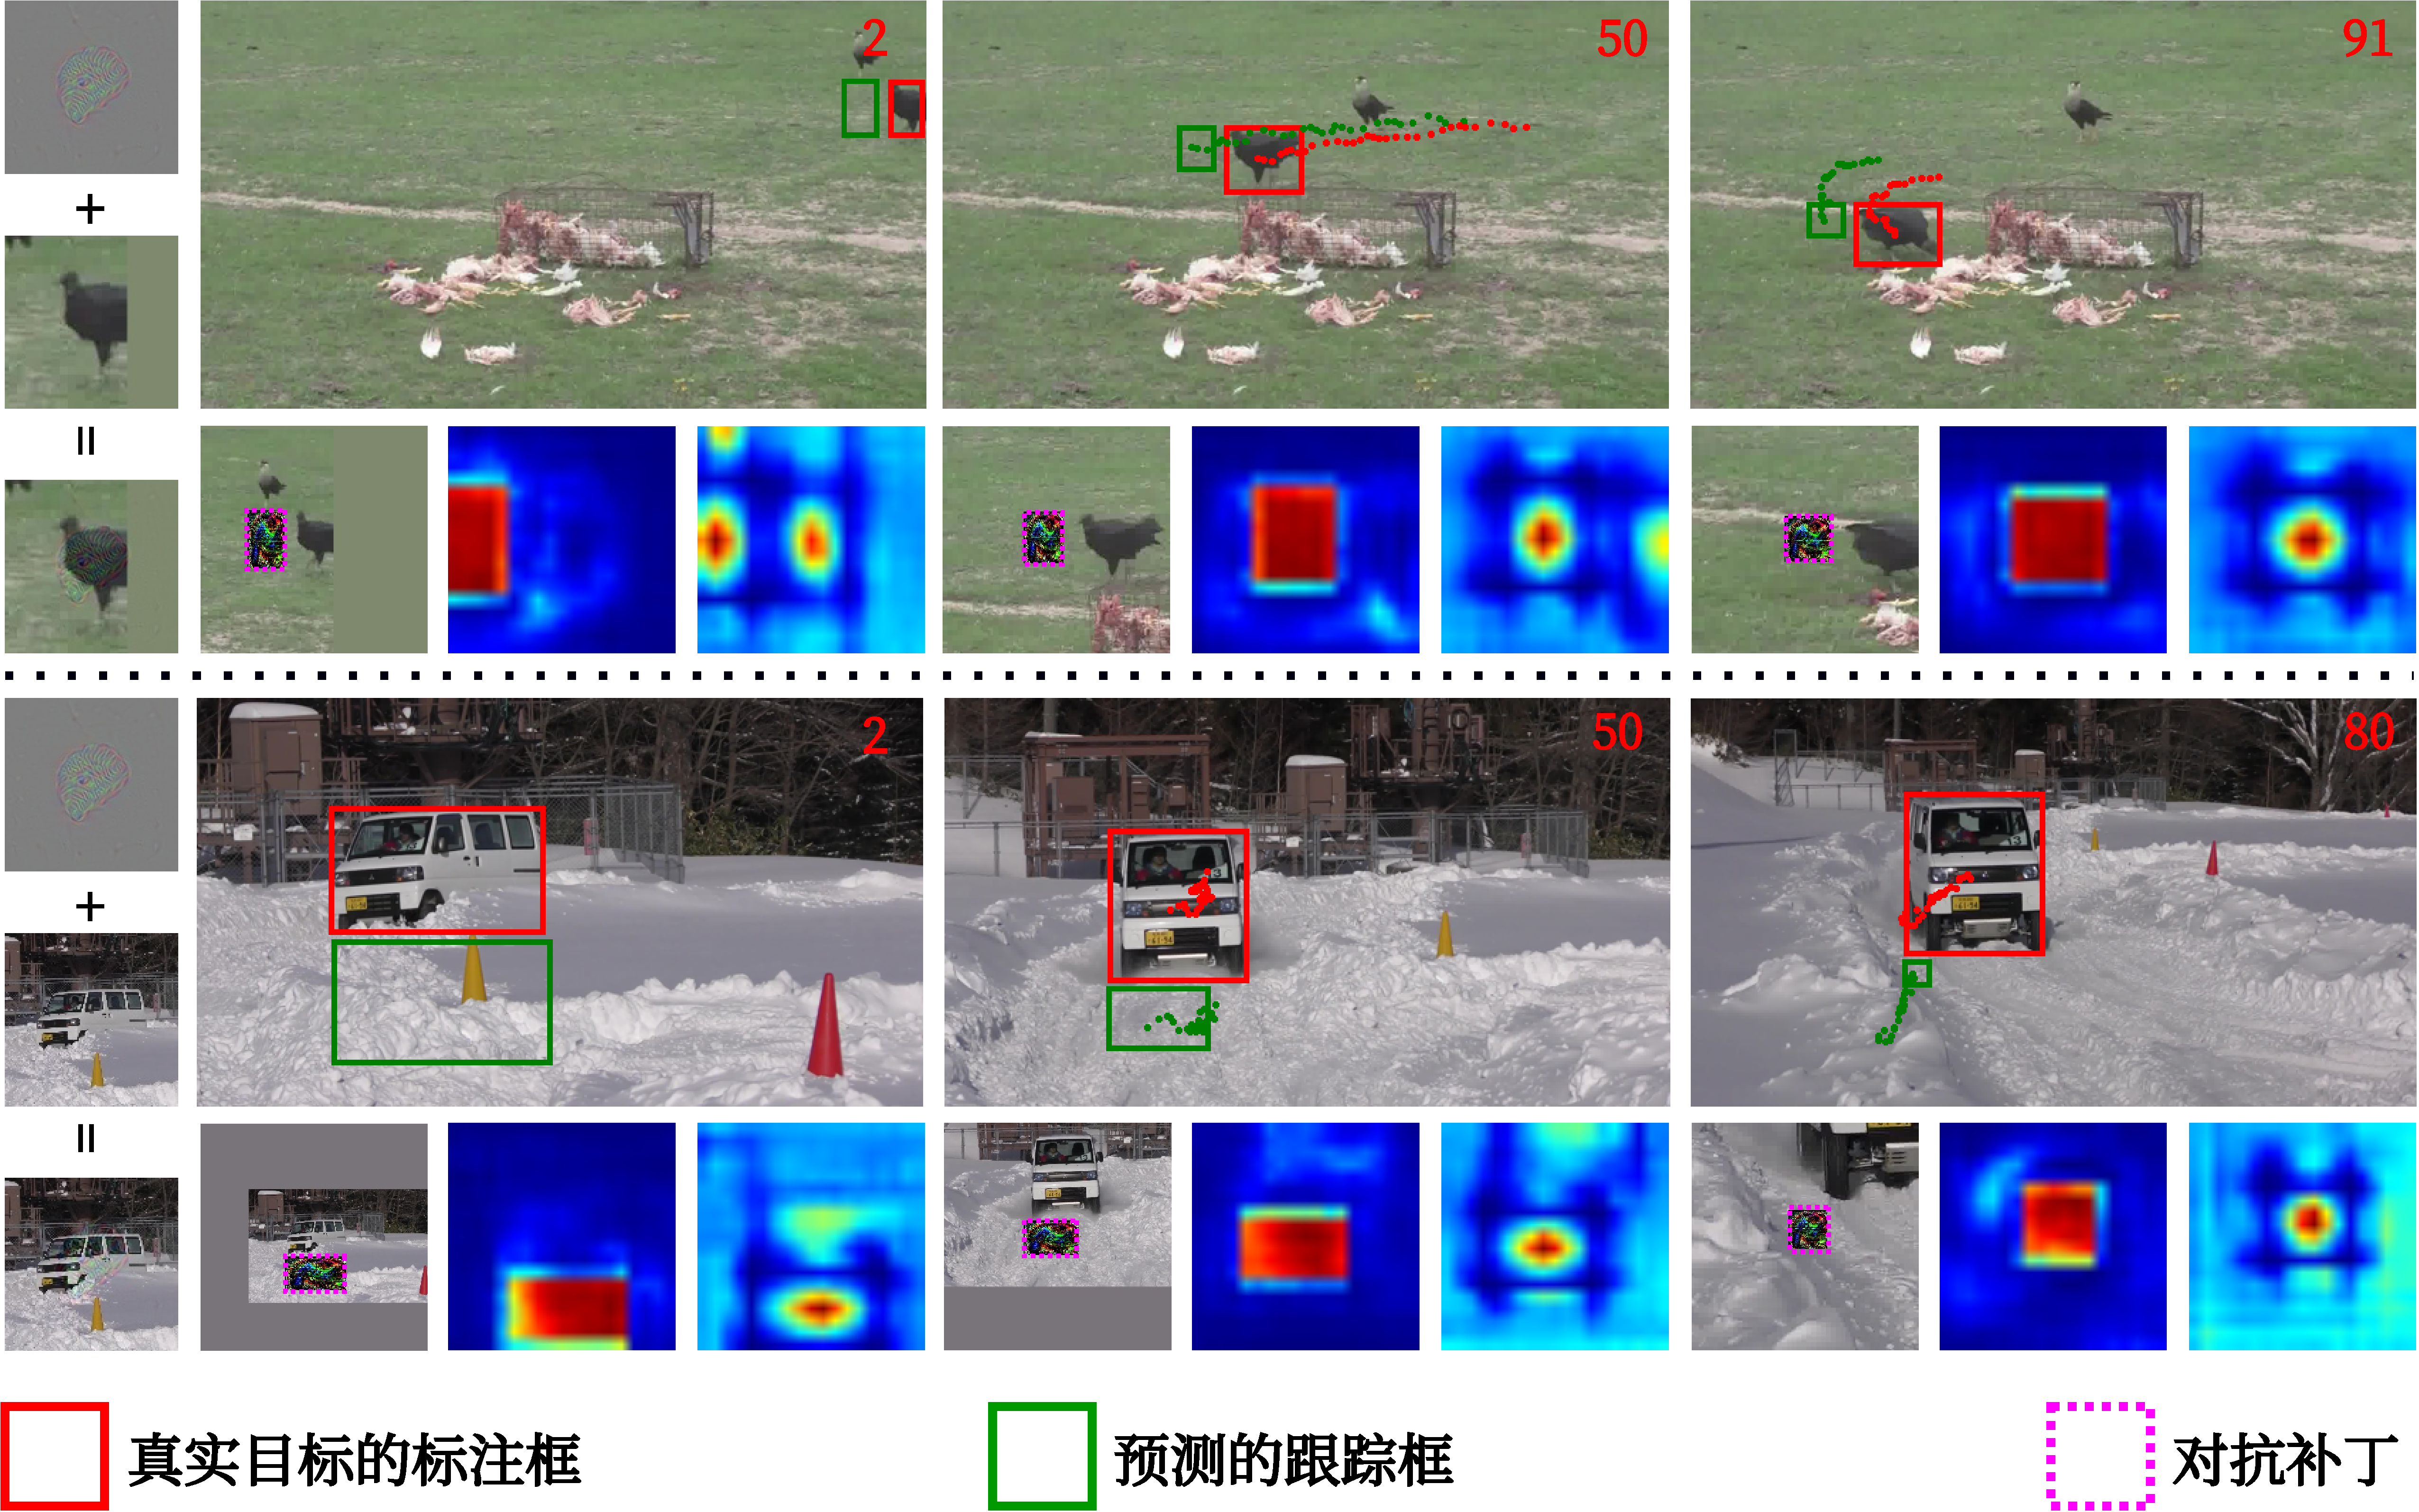
\includegraphics[width=1.0\textwidth]{Img/attack/1_v8.pdf}
\caption{在 GOT-10k 基准测试的一些示例跟踪序列上说明了我们对 SiamFC++ 的攻击。我们的方法会产生视频不可知的扰动,这实际上可以迫使 SiamFC++ 遵循复杂的轨迹,而几乎不会产生任何费用。这是通过离线训练扰动来实现的,因此跟踪器错误地认为 \textit{虚假目标} 区域包含要跟踪的对象(请参见左侧的热图)。此外,还误导了 SiamFC++ 中的质量评估分支以确认此结果(请参见右侧的热图)。\textit{虚假目标} 的大小逐渐减小。} 
%Being universal, the generated perturbations can be conveniently exploited to perturb videos on-the-fly without extra computations. 
%Red represents the ground-truth bounding box, and green represents the predicted bounding box by the tracker.
%The purple dashed box marks the universal adversarial patch. The left heatmap represents the probability of each spatial position to contain the \textit{fake target}, and the right heatmap represents the target state estimation quality.}
\label{fig:1}
\end{figure}

近来,孪生跟踪器的鲁棒性在测试其对抗攻击的脆弱性方面引起了很多关注,并且重点已转向更有效,成本更低的攻 \cite{TTP,FAN,SPARK}。尽管取得了成功,但这些攻击方法仍不适合以有限的计算资源来攻击基于小型边缘平台构建的现实世界在线跟踪系统。原因是他们仍然需要基于迭代优化或对抗性网络推论来独立地为每个视频制作扰动,为此,计算密集型跟踪系统可能无法确保计算资源的充足性。

\cite{UAP} 中提出的通用对抗性扰动(UAP)可以以与图像无关的方式从数据分布中欺骗大多数图像。UAP 具有通用性,可以方便地利用它来即时扰乱看不见的数据,而无需进行额外的计算。因此,在攻击计算资源有限的平台上部署的实时应用程序时,UAP 特别有用。但是,没有任何工作涉及使用 UAP 攻击孪生跟踪器的主题,因为很难将现有的 UAP 应用于直接攻击孪生跟踪器。主要原因在于:
\begin{itemize}
\item 大多数 UAP 是为典型的神经网络设计的,其中一个图像作为输入,而孪生网络同时接受模板图像和搜索图像。
\item 现有 UAP 方法的目标是干扰一元或单个实例的二进制模型输出,而我们需要使用通用扰动导致连体追踪器遵循指定的轨迹。
\end{itemize}

在本文中,我们进行了首次尝试,以有针对性的攻击方式发现了与最新的孪生跟踪器,即 SiamFC++ \cite{SiamFC++}无关的视频不可知的干扰。在线跟踪阶段的费用。具体来说,我们旨在通过向模板图像添加通用的不可感知的扰动并将 \textit{虚假目标}(即小的通用对抗补丁)粘贴到符合预定轨迹的搜索图像中来攻击跟踪器(如图 \ref{fig:1}),以便跟踪器输出 \textit{虚假目标} 的位置和大小,而不是实际目标。我们产生的与视频无关的扰动使扰动一个新颖的视频无需付出额外的费用,仅需进行添加和粘贴操作即可,并且不需要梯度优化或网络推理。在 OTB2015 \cite{OTB},GOT-10k \cite{GOT-10k} 和 LaSOT \cite{LaSOT} 基准测试中的实验结果证明了我们方法的有效性和效率。

\section{相关工作}

\subsection{孪生视觉跟踪}

除了基于相关过滤器的方法外,孪生视觉跟踪是基于模板匹配的跟踪的基本研究方向。两者都旨在“因果”地估计从初始视频帧裁剪的模板在后续帧中的位置。孪生跟踪器将视觉跟踪公式化为以卷积方式学习目标模板和搜索区域中候选对象之间的互相关相似性。然后,通过基于最高的视觉相似度将对象定位在搜索图像区域中来执行跟踪。此范例被表述为本地单发检测任务。

最近,一些孪生跟踪器~\cite{SiamRPN,SiamRPN++,SiamFC++} 已证明在视觉跟踪方面有显着的性能改进。
特别是,SiamRPN \cite{SiamRPN} 由一个用于特征提取的孪生子网和一个分别包含分类和回归分支的区域建议子网组成。SiamRPN++ \cite{SiamRPN++} 基于其在分类和状态估计分解中的成功经验,通过一种简单而有效的空间感知采样策略进一步突破了严格的翻译不变性的限制,并成功地训练了 ResNet 驱动的孪生跟踪器,从而显着提高了性能。除了这些基于锚的方法以外,还通过考虑无歧义评分,无目标目标规模/比率分布和估计质量评估准则,进一步设计了无锚跟踪器 SiamFC++ \cite{SiamFC++} 在我们的实验中,我们将重点放在无锚的 SiamFC++ 跟踪器上,而对我们生成的对抗攻击到以前基于锚的跟踪器的可移植性也进行了研究。

\subsection{对抗攻击}

图像分类的对抗性攻击首先在 \cite{intriguing} 中进行了研究,目的是确定现代深度网络对不可察觉的扰动的脆弱性。
%Recent studies also emerge to investigate the adversarial attacks to other diverse types of tasks such as natural language processing \cite{generating} and object detection \cite{wei2019transferable}.
可能的对抗攻击的场景可以按照不同的维度进行分类。

\textit{不可感知的扰动对抗性补丁} 难以察觉的扰动最常会使每个像素发生少量变化,并且可以使用多种优化策略来找到,例如有限内存 BFGS \cite{intriguing} 和 PGD \cite{PGD}。
与不可察觉的扰动不同,对抗性补丁对神经网络非常重要。对抗补丁可以放置在输入图像中的任何位置,以引起网络行为异常,因此通常用于通用攻击 \cite{patch}。
据我们所知,我们是第一个同时利用不易察觉的扰动和对抗性补丁来攻击目标跟踪器的方法,它们以端到端的方式共同训练。
请注意,我们的对抗性补丁程序在网络域而不是图像域中工作。在网络域的情况下,噪声可以取任何值,并且不限于图像值情况下的动态范围  \cite{karmon2018lavan}。

\textit{非针对性攻击有针对性的攻击} 在无目标攻击的情况下,对手的目标是使网络预测任何不正确的标签,而无论不正确的标签无关紧要,例如,在视觉跟踪中将对象位置估计推到真正的搜索区域之外。
但是,有针对性的攻击旨在将网络的预测更改为某些特定的目标标签。在视觉跟踪中,有针对性的攻击旨在有意驱使跟踪器按照预定的轨迹输出指定的对象位置。

\subsection{目标跟踪中的对抗攻击}

最近,对视觉跟踪任务的对抗攻击进行了多种探索。例如,PAT \cite{PAT} 通过白盒攻击生成物理对抗纹理,以引导跟踪器在被跟踪对象移到其前面时锁定该纹理。但是,PAT 通过攻击轻型深度回归跟踪器 GOTURN \cite{GOTURN} 来验证其方法,该跟踪器在现代基准上的跟踪精度较低。在本文中,我们旨在攻击最先进的孪生跟踪器。
在估计的跟踪结果中逐帧生成轻量级扰动时,RTAA \cite{RTAA} 考虑到了时间运动。但是,RTAA 仅对跟踪器执行无目标攻击,这比本文中的有针对性的攻击更具挑战性,因为我们的目标是在测试时创建任意的复杂轨迹。

遵循看起来真实的错误路径进行有针对性的攻击对于欺骗跟踪系统而不会引起现实应用程序的怀疑至关重要。
SPARK \cite{SPARK} 通过使用过去帧中的信息对孪生跟踪器进行有针对性的攻击来计算增量扰动。但是,SPARK 需要通过繁琐的迭代方案为每个搜索图像生成独特的对抗示例,这对于实时攻击在线跟踪非常耗时。\cite{TTP} 中最近的实时攻击者仅使用模板图像以一次生成的方式生成时间可传递的扰动,然后将其添加到每个搜索图像中。但是,该方法仍然需要为每个视频生成扰动,并且其有针对性的攻击设置需要从网络推理的多次运行中获得不同的扰动。当我们无法访问有限的计算资源时,就不适合攻击现实世界的在线跟踪系统。但是,在本文中,我们提出了与视频无关的扰动,该扰动允许仅通过添加和粘贴操作即可对新颖的视频进行扰动,而无需支付额外的费用。

\begin{figure}[t]
\centering
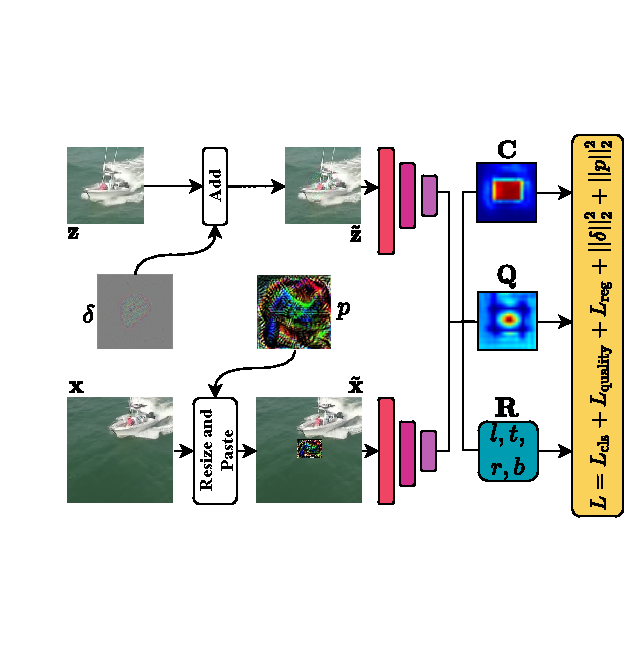
\includegraphics[width=0.75\textwidth]{Img/attack/network_v5.pdf}
\caption{所提出方法的训练流程。我们旨在为模板图像 $\textbf z$ 训练难以察觉的扰动 $\delta$ ,为搜索图像 $\textbf x$ 训练对抗性补丁 $p$ 。在将 $\delta$ 添加到 $\textbf z$ 并将 \textit{虚假目标} $p$ 粘贴到 $\textbf x$ 之后,跟踪器将输出  \textit{虚假目标} 的位置和大小,而不是实际的目标。}
\label{fig:net}
\end{figure}

\section{方法}

\textcolor{black}{在本节中,我们介绍了针对孪生跟踪器的视频不可知的定向攻击框架。我们旨在通过向模板图像添加不可察觉的扰动并将 \textit{虚假目标}(即对抗补丁)粘贴到符合预定轨迹的搜索图像中来攻击跟踪器,以便跟踪器输出位置和大小 \textit{虚假目标} 而不是真实目标。下面,我们将对 \cite{SiamFC++} 的针对性攻击正式化,然后详细介绍我们的扰动策略。}

\subsection{问题定义}

令 $V=\{I_i\}_1^T$ 表示长度为 $T$ 的视频序列的帧。
$B^{gt}=\{b^{gt}_i\}_1^T$ 用于表示目标在每一帧中的真实位置。
视觉对象跟踪旨在在给定其初始状态的情况下,在随后的帧中预测此目标的位置 $B^{pred}=\{b^{pred}_i\}_1^T$。
在 SiamFC++ 中,跟踪器首先将配对的参考框架 $I_1$ 和注释 $b_1^{gt}$ 转换为模板图像 $\textbf z$,然后将搜索帧 $I_i$ 转换为搜索图像 $\textbf x_i$ 以上一帧中估计的位置为中心。
在每个时间步,模板图像 $\textbf z$ 和搜索图像 $\textbf x_i$ 首先分别通过共享的骨干网络传递,然后,某些非共享层处理所得的特征,并按深度将其融合。明智的可分离相关性。然后,融合后的特征将用作头网络的输入,该头网络预测分类图 $\textbf{C}$,边界框回归图 $\textbf{R}$ 和质量评估图 $\textbf{Q}$ 以无锚的方式。简而言之,$\textbf C$ 编码每个空间位置包含目标的概率,$\textbf R$ 回归目标的边界框,而 $\textbf Q$ 预测目标状态估计质量。然后根据 $\textbf{C}$,$\textbf{R}$ 和 $\textbf{Q}$ 生成最终边界框。

形式上,我们的目标是为模板图像 $\textbf z$ 训练不易察觉的扰动 $\delta$,为搜索图像 $\textbf x_i$ 训练对抗性补丁 $p$ 。在将 $\delta$ 添加到 $\textbf z$ 并将虚假目标 $p$ 粘贴到 $\textbf x_i$ 之后,跟踪器将输出对抗性补丁的位置和大小,而不是实际目标(请参见图 \ref{fig:net})。
$\delta$ 和 $p$ 是通用的(即,与视频无关),这意味着扰动新颖的视频仅涉及将扰动添加和粘贴到模板和搜索图像上,而无需进行梯度优化或网络推断。

\subsection{产生视频不可知的扰动}

在本小节中,我们展示了如何为孪生跟踪器训练与视频无关的扰动 $(\delta, p)$ 在训练的第 $k$ 次迭代中,从训练数据集 $V=\{I_i\}_1^T$ 中随机选择了视频 $\mathcal V$。假设第 $k$ 次迭代的模板扰动是 $\delta_k \in \mathbb{R}^{127\times 127 \times 3}$,而对抗性补丁是 $p_k \in \mathbb{R}^{128\times 128\times 3}$。我们首先从 $V$ 中随机选择配对的帧 $I_t, I_s$。
干净的模板图像 $\textbf z\in \mathbb{R}^{127\times 127 \times 3}$ 是根据 $I_t$ 和 $b^{gt}_t$ 生成的,受干扰的模板图像为:
\begin{equation}
\tilde {\textbf z} = \textbf z + \delta_k.
\end{equation}
类似地,干净的搜索图像 $\textbf x \in \mathbb{R}^{303\times 303 \times 3}$ 是根据 $I_s$ 和 $b^{gt}_s$ 生成的。
如前所述,补丁被视为 \textit{虚假目标} 并粘贴到搜索图像中。我们将 \textit{虚假目标} 的中心位置逼近真实目标的中心位置(在64个像素的移动范围内),其中移动定义为由均匀分布生成的最大平移范围。
\textit{虚假目标} 的宽度/高度在 32 像素和 128 像素之间随机选择。
扰动的搜索图像生成如下:
\begin{equation}
\tilde{\textbf x} = A(\textbf x, p_k, (l^x, l^y), (w, h)),
\end{equation}
其中 $(l^x, l^y)$ 和 $(w, h)$ 分别表示 \textit{虚假目标} 相对于搜索图像的位置和大小。$A$ 是补丁应用程序运算符 \cite{patch},它首先将补丁 $p_k \in \mathbb{R}^{128\times 128\times 3}$ 的大小调整为 $\hat{p}_k \in \mathbb{R}^{w\times h\times 3}$,然后将调整大小的补丁 $\hat{p}_k$ 粘贴到搜索图像 $\textbf x$ 的 $(l^x,l^y)$ 位置。

随后,SiamFC++ 跟踪器 $\phi(\cdot)$ 将 $\tilde {\textbf x}$ 和 $\tilde{\textbf z}$ 作为输入,并进行如下预测:
\begin{equation}
\textbf{C, R, Q} = \phi(\tilde {\textbf x}, \tilde{\textbf z}).
\end{equation}

\textit{训练目标} 损失函数的计算如下:
\begin{equation}
\begin{array}{l}
\begin{aligned}
L&=\frac{\alpha}{N_{\mathrm{pos}}} \sum_{x, y} L_{\mathrm{cls}}\left(\textbf{C}_{x, y}, \textbf{C}_{x, y}^{*}\right) \\
&+\frac{\beta}{N_{\mathrm{pos}}} \sum_{x, y} \textbf{1}_{\left\{\textbf{C}_{x, y}^{*}>0\right\}} L_{\mathrm{quality}}\left(\textbf{Q}_{x, y}, \textbf{Q}_{x, y}^{*}\right) \\
&+\frac{\gamma}{N_{\mathrm{pos}}} \sum_{x, y} \textbf{1}_{\left\{\textbf{C}_{x, y}^{*}>0\right\}} L_{\mathrm{reg}}\left(\textbf{R}_{x, y}, \textbf{R}_{x, y}^{*}\right) \\
&+\eta \cdot ||\delta_k||_2^2 +  \sigma \cdot ||p_k||^2_2,
\end{aligned}
\end{array}
\label{eq:loss}
\end{equation}
\textcolor{black} %(SiamFC++)
{其中 $\textbf{C}_{x, y}, \textbf{R}_{x, y}, \textbf{Q}_{x, y}$ 分别表示 $\textbf{C}, \textbf{R}, \textbf{Q}$ 在位置 $(x, y)$ 的值。$\textbf{C}^*, \textbf{R}^*, \textbf{Q}^*$ 是根据 \textit{虚假目标} 的位置和大小生成的伪造标签。$\textbf 1$ 是指标函数,如果订阅中的条件成立,则取 1,否则将取 0,$N_{\mathrm{pos}}$ 表示训练阶段正样本的数量,$L_{\mathrm{cls}}$ 表示分类结果的焦点损失 \cite{focal},$L_{\mathrm{quality}}$ 表示质量评估的二元交叉熵(BCE)损失,$L_{\mathrm{reg}}$ 表示边界框回归的 IoU 损耗 \cite{iou-loss}。在SiamFC++ 之后,如果将 $(x, y)$ 视为正样本,则将 1 分配给 $\textbf{C}_{x, y}^{*}$,如果视为负样本,则分配 0。}

\begin{algorithm}[tb]
\caption{训练过程}
\label{alg:algorithm}
\textbf{输入}: 训练数据集 $\mathcal{V}$,孪生跟踪器 $\phi$ 和最大迭代次数 $N$。\\
\textbf{输出}: 微小扰动 $\delta$ 和对抗补丁 $p$。
\begin{algorithmic}[1] %[1] enables line numbers
\State 令 $k = 0$.
\While{$k < N$}
\State 随机选择一段视频 $V\in \mathcal{V}$。对应的真实标注为 $B^{gt}=\{b^{gt}_i\}^T_1$。
\State 随机选择一对帧 $I_t, I_s$ 从 $V$ 中。
\State 生成模板图像 $\textbf{z}$ 根据 $I_t$ 和 $b^{gt}_t$。
\State $\tilde{\textbf{z}} = \textbf{z} + \delta_k.$。
\State 生成搜索图像 $\textbf{x}$ 根据 $I_s$ 和 $b^{gt}_s$。
\State 计算 \textit{虚假目标} 相对于搜索图像的位置 $\{l^x, l^y, w, h\}$。
\State $\tilde{\textbf x} = A(\textbf x, p_k, (l^x, l^y), (w, h))$。
\State $\textbf{C, R, Q} = \phi(\tilde {\textbf x}, \tilde{\textbf z})$。
\State 生成虚假标签 $\textbf{C}^*,\textbf{R}^*,\textbf{Q}^*$ 使用 $\{l^x, l^y, w, h\}$。
\State 计算损失 $L(\textbf{C, R, Q}, \textbf{C}^*, \textbf{R}^*, \textbf{Q}^*)$ 使用等式 \ref{eq:loss}。
\State $\delta_{k+1} = \delta_{k} - \epsilon_1 \cdot \text{sign}(\nabla_{\delta_k}L)$。
\State $p_{k+1} = p_{k} - \epsilon_2 \cdot \text{sign}(\nabla_{p_k}L)$。
\State $k = k + 1$。
\EndWhile
\State \textbf{返回} $\delta_N, p_N.$
\end{algorithmic}
\label{alg}
\end{algorithm}

\begin{figure*}[t]
\centering
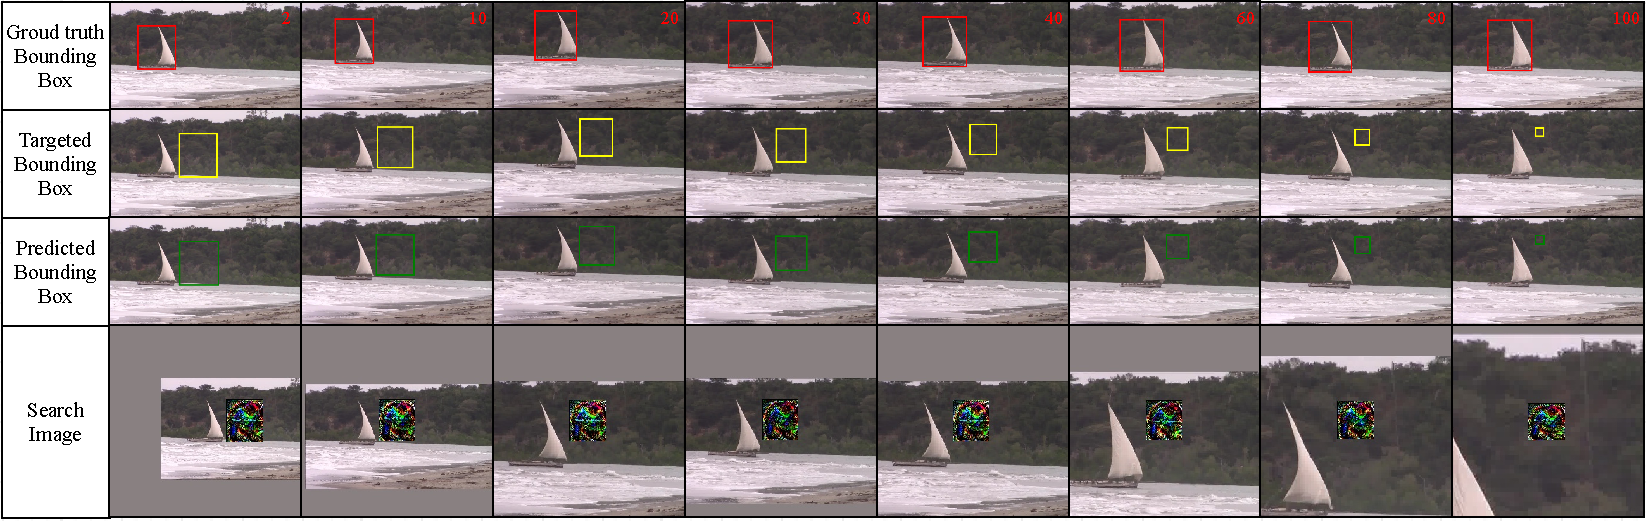
\includegraphics[width=1.0\textwidth]{Img/attack/vis_v4.pdf}
\caption{我们的目标攻击结果遵循预定义的 \textit{虚假轨迹}(由黄色的目标边界框指示)。}
\label{fig:vis}
\end{figure*}

\textit{优化} 在每个训练步骤中,扰动更新如下:
\begin{gather}
\delta_{k+1} = \delta_{k} - \epsilon_1 \cdot \text{sign}(\nabla_{\delta_k}L)\\
p_{k+1} = p_{k} - \epsilon_2 \cdot \text{sign}(\nabla_{p_k}L),
\end{gather}
其中 $\epsilon_1$ 用于确保感知不到添加到模板图像的扰动,而 $\epsilon_2$ 用于维护训练稳定性。
在训练期间,我们仅优化扰动 $(\delta, p)$ 的值,而孪生网络的参数保持不变。

我们在算法 \ref{alg} 中概述了该训练过程。

\subsection{在推理时攻击跟踪器}

一旦对扰动 $(\delta, p)$ 进行了训练,我们就可以使用它们来扰动模板图像并搜索任何新颖视频的图像进行攻击。$\delta$ 和 $p$ 都是通用的(即与视频无关),这意味着对新颖的视频进行干扰仅涉及将干扰添加和粘贴到模板和搜索图像上,而无需进行梯度优化或网络推断。
假设 $B^{fake}=\{b^{fake}_i\}_1^{T}$ 是我们希望跟踪器输出的轨迹。
在跟踪视频 $V=\{I_i\}_1^T$ 的第 $i$ 帧期间,我们需要变换边界框 $b^{fake}_i$(相对于原始帧 $I_i$)放入相对于搜索图像 $\textbf x_i$ 的框 $\hat b_i=\{l^x_i, l^y_i, w_i, h_i\}$ 中,然后根据 $\hat b_i$ 将 $p$ 粘贴到 $\textbf x_i$ :
\begin{equation}
\tilde{\textbf x}_i = A(\textbf x_i, p, (l^x_i, l^y_i), (w_i, h_i)).
\end{equation}
然后,跟踪器将 $\tilde{\textbf z}_i=\textbf z_i+\delta$ 和 $\tilde{\textbf x}_i$ 作为输入,随后的跟踪过程与 SiamFC++ 相同。

%%%%%%%%%%%%%%%%%%%%%%%%%%%%%%%
%%%%%%%%%%%%%%%%%%%%%%%%%%%%%%%
\section{实验}

\begin{table}
\centering
\begin{tabular}{c c c c c}
\toprule
\multirow{2}{*}[-2pt]{数据库} & \multirow{2}{*}[-2pt]{评价指标} & 原始图像 & \multicolumn{2}{c}{对抗图像}  \\
\cmidrule(lr){3-3} \cmidrule(lr){4-5}
                          &                         & 真实轨迹 & 真实轨迹 & 虚假轨迹     \\ 
\midrule
\multirow{2}{*}{OTB-15} 
& AO   & 0.642 & 0.035 & 0.842\\
& Precision & 0.861 & 0.048 & 0.928\\
\midrule
\multirow{2}{*}{GOT-Val} 
& SR & 0.897 & 0.023 & 0.890\\
& AO 				   & 0.760 & 0.035 & 0.818 \\
\midrule
\multirow{3}{*}{LaSOT} 
& Precision       & 0.514 & 0.013 & 0.820\\
& Norm. Prec. & 0.551 & 0.015 & 0.788\\
& AO & 0.525 & 0.022 & 0.767\\
%& Succ. rate  & 0.626 & 0.016 & 0.834\\
\midrule
\multicolumn{2}{c}{FPS} & 58 & 58 & 58\\
\bottomrule
\end{tabular}
%}
\caption{评估基准上的总体攻击结果。}
\label{tab:benchmark results}
\end{table}

\subsection{实验设置}

\textit{评估基准} 我们在几种跟踪基准,即 OTB2015 \cite{OTB},GOT-10k \cite{GOT-10k} 和 LaSOT \cite{LaSOT} 上评估针对目标攻击的视频不可知扰动。一般而言,OTB2015 是典型的跟踪基准,已被广泛用于评估中,GOT-10k 具有在幅度上更宽的对象类别的优势,LaSOT 具有更长的视频序列,平均持续时间为 84 秒。它们都遵循单次通过评估(OPE)协议,其评估方法相似,因为测量主要基于测试视频上跟踪器的成功与精确。例如,它们均根据序列的帧分数来衡量成功,在该序列中,预测矩形和地面真实矩形的交点重叠(IoU)重叠超过给定阈值,然后使用面积-曲线下(AUC)准则。由于最近证明所有测试视频帧上的 IoU 重叠平均值(AO)均等效于 AUC 标准,因此在下文中将成功度量表示为 AO。除了 AO 之外,成功率(SR)度量标准也可以直接用于测量在 GOT-10k 中给定阈值的成功跟踪帧的百分比。至于精度,它对帧的比例进行编码,对于这些比例,预测矩形的中心在地面真实中心的 20 个像素之内。由于精度度量对图像的分辨率和边界框的大小敏感,因此提出了在地面真实边界框的大小上进行归一化精度的度量,然后使用 AUC 对跟踪器进行排序,以使归一化精度介于0之间和0.5。

\textit{生成伪造的轨迹} 我们需要为每个视频预先定义特定的轨迹 $B^{fake}=\{b^{fake}_i\}_1^{T}$ ,以实现在线跟踪中的有针对性的攻击阶段,我们称之为 \textit{假轨迹}。我们用边界框地面真值将 \textit{真实轨迹} 表示为 $B^{gt}=\{b^{gt}_i\}_1^T$。
可以为每个视频手动标记任意 $B^{fake}$ ,但是,在我们的实验评估中这将非常耗时。因此,我们基于 $B^{gt}$ 生成 $B^{fake}$。具体来说,\textit{虚假轨迹} 遵循 \textit{真实轨迹},并且 $b^{fake}_i$ 和 $b^{gt}_i$ 的边界相距 16 像素。
%The size of $b^{fake}_0$ is the same as $B^{gt}_0$ and the size of $b^{fake}_i$
\textit{虚假轨迹} 的边框尺寸由 $b^{gt}_1$ 的尺寸逐渐变为 $64\times 64$。请注意,GOT-10k 测试数据的注释是保密的,因此我们仅将其验证集用于评估,并将其表示为 GOT-Val。

\textit{图像质量评估} 我们使用结构相似性(SSIM)\cite{SSIM} 来评估生成的不可感知模板扰动 $\delta$ 的质量。当 SSIM 接近 1 时很难找到(请参见表 \ref{tab:iter})。

\subsection{实施细节}

在我们的评估中,基本跟踪器 SiamFC++ \cite{SiamFC++} 的主干孪生网络采用 GoogLeNet \cite{GoogLeNet}。
我们在 Pytorch 中实施我们的方法,并使用三个 GTX 1080Ti GPU 训练我们的扰动。
我们采用 COCO \cite{COCO},ILSVRC-VID \cite{VID},及 GOT-10k \cite{GOT-10k} 与 LaSOT \cite{LaSOT} 的训练分割作为我们的训练集。
我们以 96 个图像的微型批处理(每个GPU 32个图像)训练32768次迭代的扰动。
模板扰动 $\epsilon_1$ 的学习速率设置为0.1,而对抗性补丁的学习速率为 $\epsilon_2 = 0.5$。
我们按照SiamFC ++的实践生成培训样本。
在培训和在线跟踪阶段,SiamFC++ 跟踪网络模型 \footnote{由 SiamFC++ 的作者专门使用 GOT-10k 的训练集进行训练,可以从 \url{https://drive.google.com/file/d/1BevcIEZr_kgyFjhxayOFw08DFl2u5Zi7/view} 中下载。} 是固定的,并用于整个评估。模板图片的空间尺寸设置 $127\times 127$,搜索图片的价格为 $303\times 303$。
在等式 \ref{eq:loss} 中,我们设置 $\alpha=1, \beta=1, \gamma=1, \eta=0.005$ 和 $\sigma=10^{-5}$。

\begin{table}
\centering
\begin{tabular}{ccccccc} 
\toprule
\multirow{2}{*}[-2pt]{$L_{\text{cls}}$}     & \multirow{2}{*}[-2pt]{$L_{\text{quality}}$} & \multirow{2}{*}[-2pt]{$L_{\text{reg}}$} & \multicolumn{2}{c}{虚假轨迹}          & \multicolumn{2}{c}{真实轨迹}           \\ 
\cmidrule(lr){4-5} \cmidrule(lr){6-7}
                       &                    &                    & AO                    & SR                    & AO                    & SR                     \\ 
\midrule
\checkmark   &    &    & 0.718  & 0.824    & 0.086 & 0.083   \\
   & \checkmark   &    & 0.044  & 0.044    & 0.703 & 0.842   \\
   &    & \checkmark   & 0.664  & 0.726    & 0.165 & 0.184   \\
\checkmark   & \checkmark   & \checkmark   & 0.818  & 0.890    & 0.035 & 0.023   \\ \bottomrule
\end{tabular}
%}
\caption{每项损失对 GOT-Val 的贡献。}
\label{tab:loss}
\end{table}

\subsection{评估基准的攻击结果}

\begin{figure}
\centering
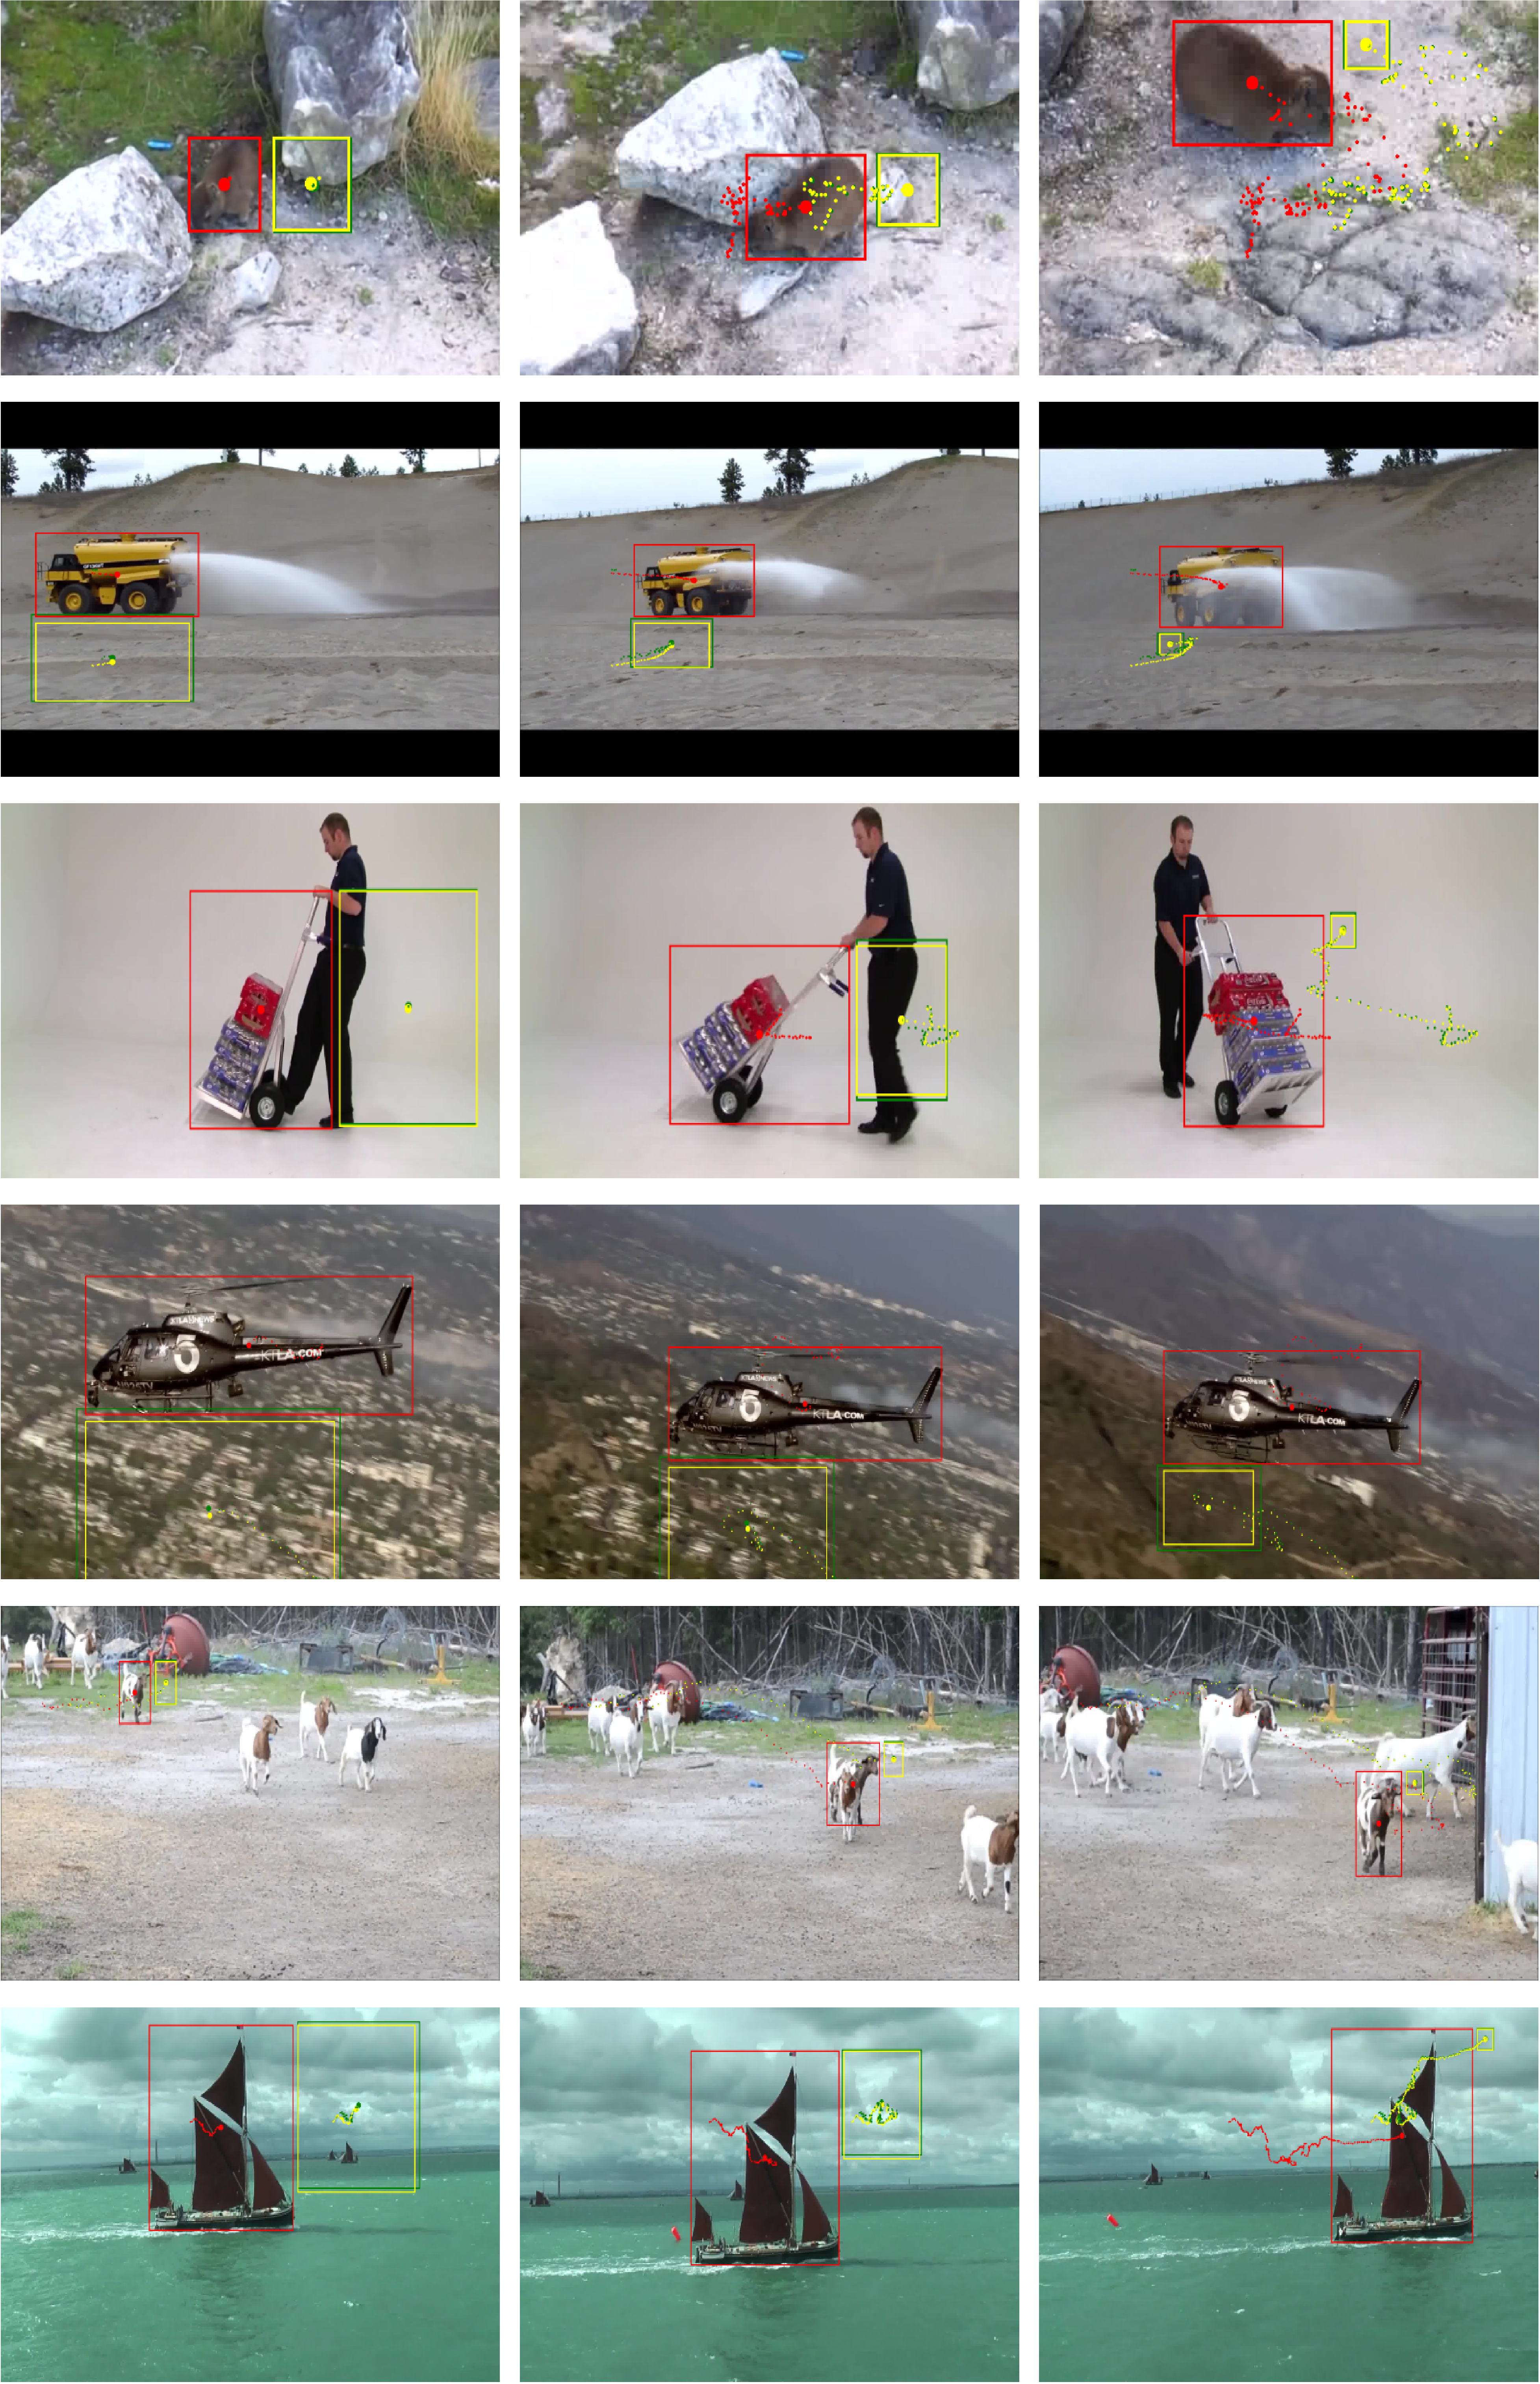
\includegraphics[width=1.0\textwidth]{Img/attack/txt_visualize.pdf}
\caption{可视化结果}
\end{figure}

\textit{总体攻击结果} 我们在评估基准上测试了针对性攻击方法的性能,并将总体结果收集在表 \ref{tab:benchmark results}中。结果表明,基本跟踪器 SiamFC++ 可以在所有评估基准上达到最先进的性能,并且可以实时运行(在 GTX 1080Ti GPU 上约为 58 fps)。但是,这种实时性能要求计算量大的跟踪系统占用大部分计算资源,因此吸引人的是开发一种几乎无成本的攻击方法来欺骗跟踪系统而不会争用资源。如表 \ref{tab:benchmark results}所示,我们的攻击方法可以满足该要求,并通过误导跟踪器遵循预定义的 \textit{虚假轨迹} 来有效地欺骗 SiamFC++ 跟踪器。此外,相对于 \textit{虚假轨迹} 而言,较高的 AO 和 Precision 性能表明在没有引起任何怀疑的情况下更有效的攻击(请参见 \ref{fig:vis})。

\begin{table*}[t]
\centering
\begin{tabular}{rrcccccccccccccccc} 
\toprule
\multicolumn{2}{r}{迭代次数}     & 1     & 2     & 4     & 8     & 16    & 32    & 64    & 128   & 256   & 512   & 1024  & 2048  & 4096  & 8192  & 16384 & 32768  \\ 
\midrule
\multirow{2}{*}{虚假轨迹} & AO    & 0.002 & 0.002 & 0.002 & 0.002 & 0.002 & 0.003 & 0.007 & 0.042 & 0.299 & 0.668 & 0.746 & 0.781 & 0.798 & 0.820 & 0.821 & 0.818  \\
                                 & SR    & 0.000 & 0.000 & 0.000 & 0.000 & 0.000 & 0.001 & 0.005 & 0.044 & 0.335 & 0.749 & 0.822 & 0.855 & 0.872 & 0.895 & 0.897 & 0.890  \\ 
\midrule
\multirow{2}{*}{真实轨迹} & AO    & 0.757 & 0.756 & 0.757 & 0.757 & 0.758 & 0.759 & 0.753 & 0.720 & 0.474 & 0.150 & 0.095 & 0.071 & 0.041 & 0.032 & 0.032 & 0.035  \\
                                 & SR    & 0.894 & 0.891 & 0.893 & 0.891 & 0.893 & 0.896 & 0.888 & 0.852 & 0.559 & 0.164 & 0.098 & 0.066 & 0.031 & 0.021 & 0.022 & 0.023  \\ 
\midrule
\multicolumn{2}{r}{SSIM of $\delta$}                        & 1.00  & 1.00  & 1.00  & 1.00  & 0.99  & 0.99  & 0.97  & 0.93  & 0.86  & 0.86  & 0.87  & 0.88  & 0.88  & 0.88  & 0.88  & 0.88   \\
\multicolumn{2}{r}{MSE}                         & 0.51  & 0.26  & 0.32  & 0.37  & 0.48  & 0.84  & 2.03  & 5.65  & 15.10 & 25.43 & 23.70 & 21.89 & 20.69 & 20.49 & 20.03 & 20.87  \\
\bottomrule
\end{tabular}
\caption{训练迭代次数对 GOT-Val 的影响。}
\label{tab:iter}
\end{table*}

\begin{table}[t]
\centering
\begin{tabular}{c cc cc cc} 
\toprule
\multirow{3}{*}[-6pt]{主干网络} & \multicolumn{2}{c}{原始视频}    & \multicolumn{4}{c}{扰动视频}                                        \\ 
\cmidrule(lr){2-3} \cmidrule(lr){4-7}
                          & \multicolumn{2}{c}{真实轨迹} & \multicolumn{2}{c}{真实轨迹} & \multicolumn{2}{c}{虚假轨迹}  \\ 
\cmidrule(lr){2-3} \cmidrule(lr){4-7}
                          & AO    & SR                           & AO    & SR                           & AO    & SR                           \\ 
\midrule
GoogLeNet                 & 0.760 & 0.897                        & 0.035 & 0.023                        & 0.818 & 0.890                        \\
AlexNet                   & 0.720 & 0.850                        & 0.196 & 0.227                        & 0.572 & 0.640                        \\
ShuffleNet                & 0.766 & 0.888                        & 0.554 & 0.656                        & 0.135 & 0.134                        \\
\bottomrule
\end{tabular}
%}
\caption{可转移到 GOT-Val 上不同的主干。}
\label{tab:backbone}
\end{table}

\begin{table}
\centering
\begin{tabular}{ccccc} 
\toprule
\multirow{2}{*}[-2pt]{跟踪器} & \multicolumn{2}{c}{原始视频} & \multicolumn{2}{c}{对抗视频}  \\
\cmidrule(lr){2-3} \cmidrule(lr){4-5}
                          & AO & Precision              & AO & Precision                   \\
\midrule
SiamRPN++                 & 0.676   & 0.879                  & 0.518   & 0.691                       \\
SiamRPN                   & 0.666   & 0.876                  & 0.379   & 0.506                       \\
\bottomrule
\end{tabular}
%}
\caption{在 OTB2015 上可转移到不同的跟踪体系结构。}
\label{tab:arch}
\end{table}

\textit{消融研究:培训损失的影响} 我们实施了一系列实验来分析和评估每个损失成分的贡献。
在表 \ref{tab:loss}中,我们报告了关于 GOT-Val 的结果,这些结果与在等式中用损失项的不同组合训练的不同扰动有关。(等式\ref{eq:loss})
总而言之,所有损失项都是有益的,而分类项比质量评估项更重要。

\textit{消融研究:训练迭代的影响} 如表 \ref{tab:iter}所示,经过大约 30000 次训练迭代后,所产生的扰动会欺骗 GOT-Val 中的大多数目标。关于 \textit{虚假轨迹} 的 AO 从 0.760 下降到 0.035。我们注意到,在训练周期开始时(训练迭代次数小于2048),AO 的降低明显快于后期。这证明了我们的端到端训练流水线的快速收敛能力,同时产生了对抗性扰动。

\subsection{传输性分析}

\textit{向不同骨干的传输能力} 当将扰动应用于 SiamFC++ 的另外两个不同的主干,即,ShuffleNet \cite{ShuffleNet} 和 AlexNet \cite{AlexNet}。
实验结果显示在表 \ref{tab:backbone} 中。对于 SiamFC++-AlexNet,关于 \textit{真实轨迹} 的AO从0.72下降到 0.196。但是,我们的扰动不能很好地推广到 SiamFC++-ShuffleNet,我们推测这是由于 ShuffleNet 中的特定组卷积和通道洗牌操作所致。

\textit{不同跟踪架构的迁移能力} 当将扰动应用于另外两个基于锚的最新跟踪器时,我们评估攻击的可传递性:基于 AlexNet 的 SiamRPN \cite{SiamRPN} 和基于 ResNet 的 SiamRPN++ \cite{SiamRPN++},以验证对不同跟踪体系结构的可移植性。
SiamRPN 使用 RPN 网络在响应图上执行位置回归和目标分类。 SiamRPN++ 在使用 ResNet 主干进行有效训练的基础上,执行分层和深度聚合,以提高准确性。实验结果显示在表 \ref{tab:arch} 中。在 SiamRPN 的情况下,相对于 \textit{真实轨迹} 的 AO 从 0.666 降低到 0.379,而 SiamRPN++ 的性能从 0.676 降低到 0.518。结果表明,即使将生成的扰动应用于基于锚的跟踪器,我们的攻击也可以很好地转移到不同的跟踪体系结构。

\subsection{与其他方法的比较}

我们将我们的方法的攻击性能与最新的有前途的攻击方法进行比较,即基于 AlexNet 的非目标攻击方法 CSA \cite{CSA},和其他两种有目标攻击方法:基于 AlexNet 的 FAN \cite{FAN} 和基于 ResNet-50 的 TTP \cite{TTP}。
我们在表 \ref{tab:untargeted} 中报告相对于 \textit{真实/虚假轨迹} 的精度得分。
除了单纯的添加和粘贴操作外,我们的方法在性能上明显优于其他方法,而且不需要梯度优化或网络推断。

\section{结论}

在本文中,我们提出了一种针对孪生跟踪器的视频不可知的有针对性的攻击方法。
我们旨在通过向模板图像添加不可察觉的扰动并将 \textit{虚假目标}(即小的对抗补丁)粘贴到符合预定轨迹的搜索图像中来攻击跟踪器,以便跟踪器输出位置和 \textit{虚假目标} 的大小,而不是实际目标。由于具有通用性,因此可以方便地利用生成的扰动来即时扰动视频,而无需进行额外的计算。
在几个流行的数据集上进行的实验表明,我们的方法可以有效地以有针对性的攻击方式欺骗孪生跟踪者。

\begin{table}[t]
\centering
\begin{tabular}{@{}ccccccc@{}}
\toprule
\multirow{2}{*}[-2pt]{方法} & \multirow{2}{*}[-2pt]{跟踪器} & \multirow{2}{*}[-2pt]{攻击时间(毫秒)} & \multirow{1}{*}[-2pt]{原始视频} && \multicolumn{2}{c}{对抗视频} \\
\cmidrule{4-4} \cmidrule{6-7}
 &  &  & 真实轨迹 & & 真实轨迹 & 虚假轨迹 \\ \midrule
CSA & SiamRPN & 4720 & 0.851 & & 0.458 & - \\
FAN & SiamFC & 10 & 0.720    & & 0.180&0.420 \\
TTP & SiamRPN++ & 8 & 0.910  && 0.080&0.692 \\
\midrule
Ours & SiamFC++ & 0 & 0.861  & & 0.048&0.928 \\ \bottomrule
\end{tabular}%
\caption{关于 OTB2015 上 \textit{真实/虚假轨迹} 的精确度得分。}
\label{tab:untargeted}
\end{table}